\section{Cubic divisor growth and canonical reconstruction}\label{sec:reconstruction}
\noindent\textit{Source anchor D: v0.14. This section gives the analytic arguments in rendered mathematical notation, incorporating the fresh audit's precise finite-theta grammar and the distinct cutoff symbol $R_*$.}

\subsection{Explicit three-dimensional families}
For integers $n\ge1$, $1\le i,j,k\le n$, define
\begin{equation}\label{eq:families}
 Z_{i,j,k}^{(n)}=\lambda(-i,j,5(n+k)),\qquad
 P_{i,j,k,r}^{(n)}=\lambda(-i,j,5(n+k)-r),\quad 1\le r\le4.
\end{equation}
Every such triple has $a<0$, $b>0$, $3c>2b$. Hence $p>0$ and the bracket in \eqref{eq:complete-divisor} is one. The $Z$ points have order four and the $P$ points have order minus one. Rational independence makes the parameter map injective. The pole indices are distinct because $5(k-k')=r-r'$ forces both sides to vanish; the zero and pole families are disjoint by $c$ modulo five.
\begin{theorem}[Two-sided cubic growth]\label{thm:cubic-growth}
Let $n_+(r)$ and $n_-(r)$ count the zeros and poles of $R$ in $|z|\le r$, with multiplicity. Then
\[
 n_+(r)=\Theta(r^3),\qquad n_-(r)=\Theta(r^3),\qquad
 n_D(r):=n_+(r)+n_-(r)=\Theta(r^3).
\]
In particular, for $K_0=(|\tau|+|s|+2)/|\beta|$,
\[
 n_+(K_0n)\ge4n^3,\qquad n_-(K_0n)\ge4n^3.
\]
These are unsigned counts; no cubic lower bound for a signed zero-minus-pole mass is asserted.
\end{theorem}
\begin{proof}
In \eqref{eq:families}, $|a|,b\le n$ and $0<c\le10n$. The triangle inequality places every displayed point in $|z|\le K_0n$. There are $n^3$ distinct zero points of multiplicity four and $4n^3$ distinct simple poles.

For the upper bound first consider $F$. A nonzero coefficient in \eqref{eq:base-divisor} has $H(a)\ne H(b)$, so the imaginary parts of $a\tau$ and $bs$ have the same sign. Therefore
\[
 |\Im(a\tau+bs)|=|a|\Im t+|b|\Im s.
\]
A bounded complex radius bounds $|a|$ and $|b|$ by $O(r)$; the real part then bounds $|c|$ by $O(r)$. There are $O((1+r)^3)$ triples, and absolute weights are at most four. The seven translated numerator factors and the scaled denominator in \eqref{eq:p7} give a finite union of such cone supports and cannot increase this order. Combining the upper bound with the explicit lower families, choosing $n=\lfloor r/K_0\rfloor$, proves the assertion for all sufficiently large $r$.
\end{proof}

\subsection{A worked ceiling calculation}
At $n=1$ the family consists of the zero $\lambda(-1,1,10)$ and four poles $\lambda(-1,1,c)$, $c=6,7,8,9$. The exact digit data are
\begin{center}
\begin{tabular}{rrrrr}\toprule
$c$&$3c-2$&$p=\lceil(3c-2)/7\rceil$&$k=7p+2-3c$&$m_\lambda$\\\midrule
6&16&3&5&$-1$\\
7&19&3&2&$-1$\\
8&22&4&6&$-1$\\
9&25&4&3&$-1$\\
10&28&4&0&$4$\\\bottomrule
\end{tabular}
\end{center}
For example, the zero has integral lift $(\widehat a,\widehat b,\widehat c)=(4,9,5)$, so $H(4)-H(9)-H(-1)+H(1)=1$ and $w(10)=4$. The $c=6$ pole has lift $(3,7,17)$ and $w(6)=-1$. This finite example illustrates the exact global formula; it does not establish the universal statement by sampling. The same construction at $n=3$ has 27 zero points and 108 pole points, each side with total multiplicity 108.
\begin{figure}[htbp]\centering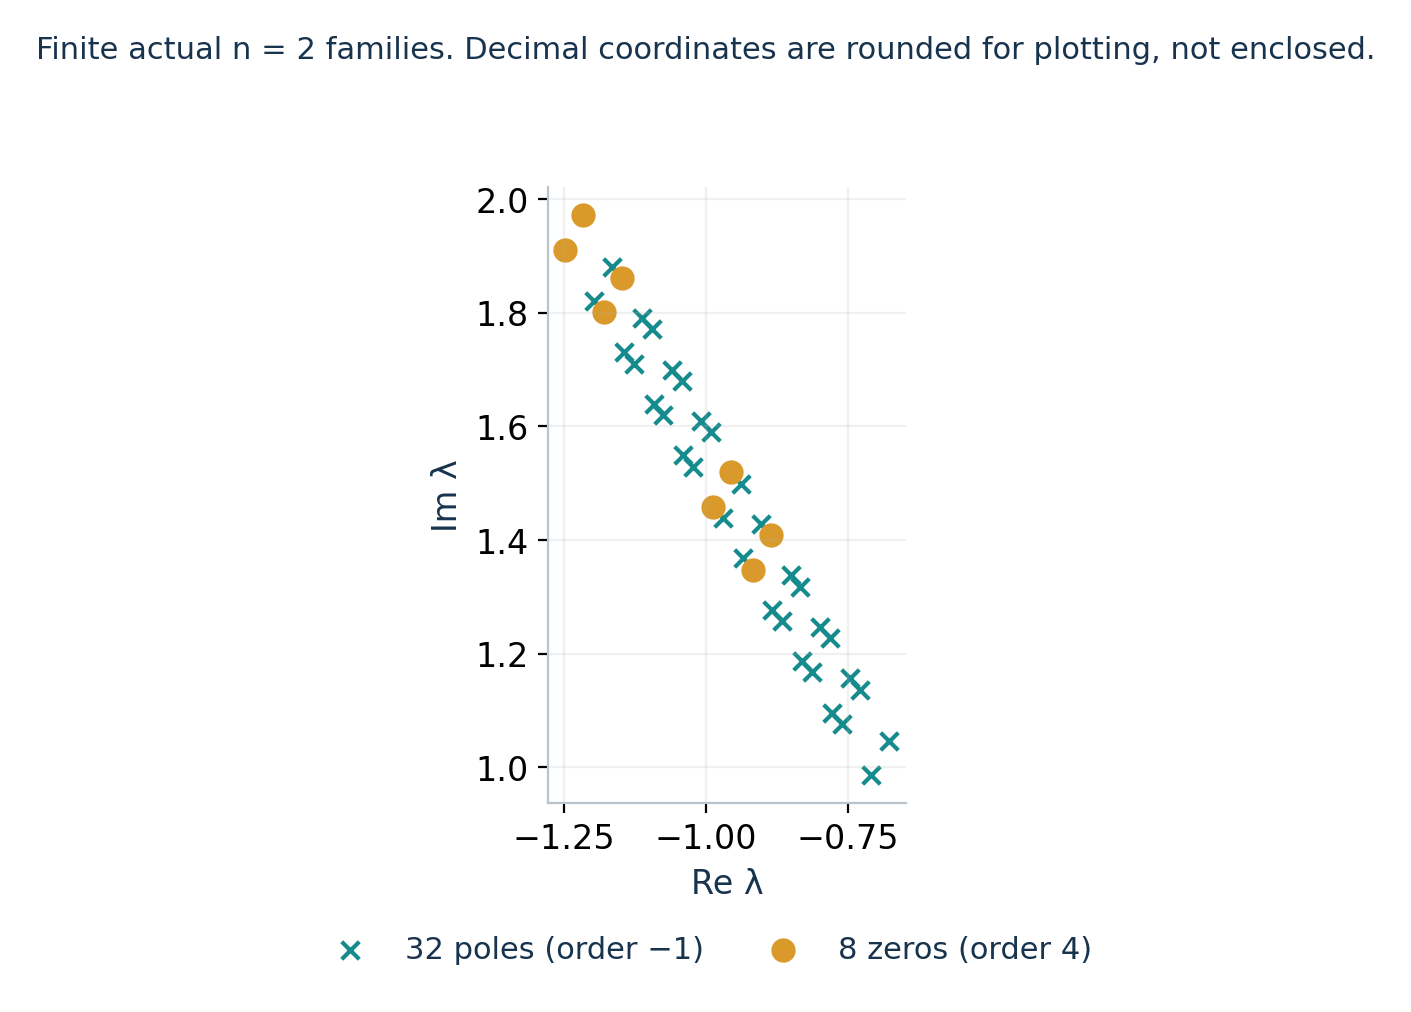
\includegraphics[width=.8\linewidth]{figures/08_complex_families.png}\caption{The actual $n=2$ divisor families have eight order-four zeros and 32 simple poles. Drawing coordinates are rounded; the cubic-growth proof uses the exact integer parametrization for all $n$.}\label{fig:family}\end{figure}

\subsection{The precise finite-theta obstruction}
\begin{theorem}[Fixed affine finite-theta class]\label{thm:theta-obstruction}
Fix finitely many symmetric period matrices $\Omega_\ell$ with positive-definite imaginary parts $\Im\Omega_\ell$, affine maps $z\mapsto A_\ell z+b_\ell$, and finite derivatives of their Riemann theta restrictions. Let $P,Q$ be nonzero entire functions formed by finite polynomial expressions in these restrictions, derivatives and polynomials in $z$. Let $u$ be a single global nowhere-zero entire function. Every meromorphic function
\[
 u(z)\frac{P(z)}{Q(z)}
\]
has zero and pole counts $O(r^2)$. Thus $R$ is not representable in this class.
\end{theorem}
\begin{proof}
For $Y=\Im\Omega>0$, the defining theta series has terms bounded by
\[
 \exp\{-\pi n^TYn+2\pi\|n\|\,\|\Im(Az+b)\|\}.
\]
Completing the square, and absorbing half of the positive quadratic form into a convergent Gaussian sum, gives $C\exp(C'|z|^2)$ for a fixed affine restriction. Cauchy estimates on fixed-radius circles give the same form for each fixed derivative. Finite sums, products and polynomial factors preserve this bound. Jensen's formula \cite{Jensen} applied about a point where $P$ is nonzero, using an outer circle of twice the radius, bounds its zero count by $O(r^2)$; the same holds for $Q$. Cancellation only decreases their divisor counts. The factor $u$ contributes no finite divisor. Theorem~\ref{thm:cubic-growth} contradicts this bound for $R$.
\end{proof}
The single global unit in this grammar cannot be moved inside arbitrary sums: $1+e^{z^3}$ has cubically many zeros and would invalidate that enlarged claim. The theorem concerns fixed finite dimensions and affine one-dimensional restrictions. It leaves infinite products, nonlinear arguments, varying period matrices, nontrivial gerbe transition data and special-value identities at $1/3$ outside its scope.

\subsection{The genus-three divisor product}
Let $D=\{\lambda:m_\lambda\ne0\}$; zero is not in $D$. Define
\begin{equation}\label{eq:WD}
 E_3(w)=(1-w)e^{w+w^2/2+w^3/3},\qquad
 W_D(z)=\prod_{\lambda\in D}E_3(z/\lambda)^{m_\lambda}.
\end{equation}
Negative exponents mean the quotient of the separate positive and negative entire products.
\begin{theorem}[Canonical regularizer and absolute genus]\label{thm:regularizer}
The products defining $W_D$ converge normally on compact sets away from their poles, and
\[
 \operatorname{div}W_D=\operatorname{div}R,\qquad W_D(0)=1,\qquad
 (\log W_D)^{(j)}(0)=0\quad(1\le j\le3).
\]
Genus three is sufficient and minimal for this ungrouped absolute construction. Special signed groupings are not excluded.
\end{theorem}
\begin{proof}
The cubic upper bound gives $\sum_D|m_\lambda|/|\lambda|^4<\infty$, by partial summation or dyadic shells. For $|w|<1$,
\[
 \log E_3(w)=-\sum_{k\ge4}\frac{w^k}{k}.
\]
On each fixed compact set the tail logarithms are thus absolutely and uniformly summable. The finitely many remaining factors supply exactly the stated orders, and each factor has its first three logarithmic jets zero at the origin. Normal convergence justifies taking these jets termwise.

The lower bound $n_D(r)\ge c r^3$ yields divergence of $\sum_D|m_\lambda|/|\lambda|^3$: partial summation contains $3\int n_D(r)r^{-4}\,dr$, which diverges logarithmically. For a fixed $z\ne0$,
\[
 \log E_2(z/\lambda)=-\frac{z^3}{3\lambda^3}+O(|\lambda|^{-4}).
\]
Its weighted absolute logarithm sum diverges, because the fourth-power remainder is summable. This proves failure of ungrouped absolute genus two, without a claim about cancellations in specially grouped signed products.
\end{proof}
\begin{proposition}[Explicit analytic tail]\label{prop:tail}
If $n_D(r)=\sum_{|\lambda|\le r}|m_\lambda|\le Ar^3$ for all $r\ge R_*$, then for $T\ge R_*$ and $|z|\le T/2$,
\begin{equation}\label{eq:tail}
 \sum_{|\lambda|>T}\frac{|m_\lambda|}{|\lambda|^4}\le\frac{4A}{T},
 \qquad |\log W_{D,>T}(z)|\le\frac{2A|z|^4}{T}.
\end{equation}
\end{proposition}
\begin{proof}
Partial summation gives the first upper bound by dropping its nonpositive boundary term and using $4\int_T^\infty Ar^3r^{-5}\,dr=4A/T$. For the tail factors the canonical branch satisfies $|\log E_3(w)|\le |w|^4/[4(1-|w|)]\le |w|^4/2$, proving the second inequality. The condition $|z|\le T/2$ keeps these tail factors away from zeros and fixes the logarithm through its power series.
\end{proof}
This is an analytic bound conditional on an explicit counting constant $A$ and cutoff $R_*$. A bounded integer search alone does not certify those infinite-support hypotheses. No evaluated numerical enclosure of $W_D(1/3)$ is claimed here.

\subsection{The fourth logarithmic derivative fixes the remaining degree}
\begin{theorem}[Cubic-exponential reconstruction]\label{thm:reconstruction}
For the actual correction $R$,
\begin{equation}\label{eq:fourth}
 (\log R)^{(4)}(z)=-6\sum_{\lambda\in D}\frac{m_\lambda}{(z-\lambda)^4},
\end{equation}
locally normally away from $D$. Consequently
\begin{equation}\label{eq:cubic-reconstruction}
 R(z)=R_0\exp(\alpha_1z+\alpha_2z^2+\alpha_3z^3)W_D(z),\qquad
 \alpha_j=\frac{(\log R)^{(j)}(0)}{j!}.
\end{equation}
The logarithmic derivatives are branch independent.
\end{theorem}
\begin{proof}
The notation $(\log R)^{(4)}$ means the third derivative of $R'/R$, a single-valued meromorphic function. The sine partial fractions \cite{DLMFSine} give
\[
 \frac{d^4}{dw^4}\log(1-e^{2\pi iw})
 =-6\sum_{n\in\mathbb Z}(w-n)^{-4}.
\]
The linear exponential factor relating $1-e^{2\pi iw}$ to $\sin\pi w$ has zero fourth logarithmic derivative. Apply this identity to each factor of the defining double gamma products. Their three-index cone supports have $O(r^3)$ counting. Initially work off the union of the individual gamma-factor divisors. The fourth-power sums are locally absolutely convergent there; rearrangement, multiplication by the argument scale $\beta$ and cancellation of multiplicities are legitimate. After coefficient cancellation, meromorphic continuation gives \eqref{eq:fourth} on $\mathbb C\setminus D$, including points where individual singularities canceled. A conditionally convergent third-power sum is never used.

The canonical factor satisfies $(\log E_3(z/\lambda))^{(4)}=-6/(z-\lambda)^4$, so the same identity holds for $W_D$. Its divisor agrees with that of $R$. Thus $R/W_D$ extends to a nowhere-zero entire function, and on the simply connected plane has an entire logarithm $h$. The fourth derivative of $h$ vanishes, hence $h$ is a polynomial of degree at most three. Its value at zero is fixed by $R_0$, and the vanished canonical jets identify the coefficients in \eqref{eq:cubic-reconstruction}.
\end{proof}
Divisor matching alone would give $e^{h(z)}$ for an arbitrary entire $h$. The fourth-log identity is the extra analytic statement forcing a cubic polynomial; no unproved finite-order estimate for the ratio is used.
\begin{figure}[htbp]\centering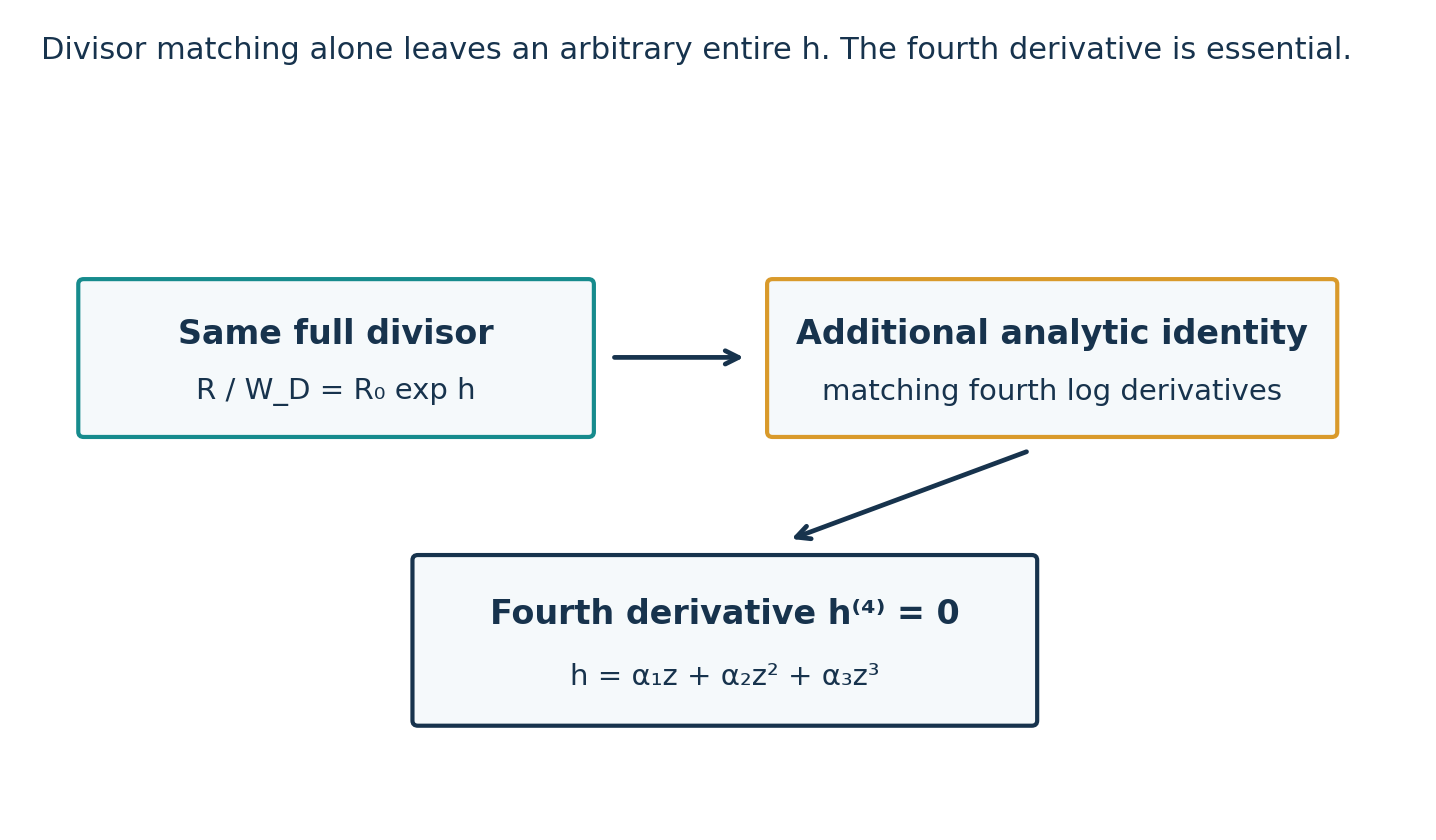
\includegraphics[width=.92\linewidth]{figures/13_ambiguity.png}\caption{The logical role of the fourth logarithmic derivative. Matching every divisor order makes the ratio a holomorphic unit; the additional analytic identity fixes the remaining exponent to degree at most three.}\label{fig:ambiguity}\end{figure}

\subsection{Reflection fixes the quadratic coefficient}
The product and continuation convention yield
\[
 F(z)F(-z)=\frac{q_t(z)}{q_s(z)},\qquad
 \frac{F(w+7\delta)}{F(w)}=\frac{q_s(w)}{q_t(w)q_t(w+s)}.
\]
Pair the labels $k$ and $7-k$ in $P_7(z)P_7(-z)$. For $1\le k\le6$,
\[
 F(z+k\delta)F(-z+(7-k)\delta)=q_t(z+k\delta-s)^{-1}.
\]
The unpaired $k=0$ term retains $q_t(z)/q_s(z)$. Dividing by the reflected denominator gives
\begin{equation}\label{eq:reflection}
 R(z)R(-z)=T(z):=
 \frac{q_t(z)q_s(\beta z)}{q_s(z)q_t(\beta z)}
 \prod_{k=1}^{6}q_t(z+k\delta-s)^{-1}.
\end{equation}
Its apparent singularities at zero are removable, and $T(0)=R_0^2$.

Let $L_t=(q_t'/q_t)'$ and $S_t=\wp_t(1/5)+\wp_t(2/5)$. The normalized theta formula gives
\[
 L_t(z)=-4z^{-2}+2S_t+O(z^2),\qquad S_s=\rho^2S_t.
\]
Since $7\delta-2s=-t+4$, evenness and $t$-periodicity pair the six translated $L_t$ terms. Using $s=u_0+3\delta-2$, their sum is $2\sum_{j=0}^{2}L_t(u_j)$. The second logarithmic derivative of \eqref{eq:reflection} cancels all $z^{-2}$ terms, leaving
\[
 (\log T)''(0)=2(1-\beta^2)(1-\rho^2)S_t-2\sum_{j=0}^{2}L_t(u_j).
\]
The left side is $4\alpha_2$. Therefore
\begin{equation}\label{eq:alpha2}
 \boxed{\alpha_2=\frac12\left[(1-\beta^2)(1-\rho^2)S_t-
 \sum_{j=0}^{2}L_t(u_j)\right].}
\end{equation}
The factor $1/2$ is fixed by reflection and is not a numerical fit.

\subsection{The period-one transition fixes the cubic coefficient}
The points $0,1,1/3$ are regular and nonzero for $R$ and $W_D$. For $1$, \eqref{eq:K} has nonzero factors at zero. For $1/3$, $\beta/3=-5s-2/3$, whose rational coordinate is not a rational fifth; rational independence excludes a singular lattice point. Define
\begin{equation}\label{eq:BD}
 B_D(1)=(\log W_D)''(1)
 =\sum_{\lambda\in D}m_\lambda\left[-\frac1{(\lambda-1)^2}
 +\frac1{\lambda^2}+\frac2{\lambda^3}\right].
\end{equation}
The combined summand is $O(|\lambda|^{-4})$, so this is an absolutely convergent sum. Its terms must remain combined; the separately divergent lower-power sums are not substituted. Taking two logarithmic derivatives of \eqref{eq:cubic-reconstruction} at the transition \eqref{eq:K} gives
\[
 (\log K)''(0)=6\alpha_3+B_D(1).
\]
Since $L_t$ is even,
\begin{equation}\label{eq:alpha3}
 \boxed{\alpha_3=-\frac16\left[\beta^2\sum_{r=1}^{15}L_t(rs)+B_D(1)\right].}
\end{equation}
Evaluating the period-one ratio also determines
\begin{equation}\label{eq:expalpha1}
 e^{\alpha_1}=\frac{K(0)e^{-\alpha_2-\alpha_3}}{W_D(1)}.
\end{equation}
This evaluates the exponential, without choosing an unjustified principal logarithm.

\begin{theorem}[Branch-free special cube]\label{thm:cube}
The exact analytic reconstruction at $z=1/3$ is
\begin{equation}\label{eq:cube}
 \boxed{R(1/3)^3=R_0^3K(0)\frac{W_D(1/3)^3}{W_D(1)}
 \exp\left(-\frac23\alpha_2-\frac89\alpha_3\right).}
\end{equation}
The right side consists of specified theta values and derivatives, algebraic period data and absolutely convergent genus-three products and sums. It contains no gamma value, arbitrary normalization scalar or new root choice.
\end{theorem}
\begin{proof}
Cube \eqref{eq:cubic-reconstruction} at $1/3$ to get $R_0^3e^{\alpha_1+\alpha_2/3+\alpha_3/9}W_D(1/3)^3$, then substitute \eqref{eq:expalpha1}. The resulting exponents are $-2\alpha_2/3$ and $-8\alpha_3/9$.
\end{proof}
This is an analytic representation by an infinite transcendental product. It does not identify that product with a class-field value or prove $U_\Gamma=U_{\rm alg}$.
\begin{figure}[htbp]\centering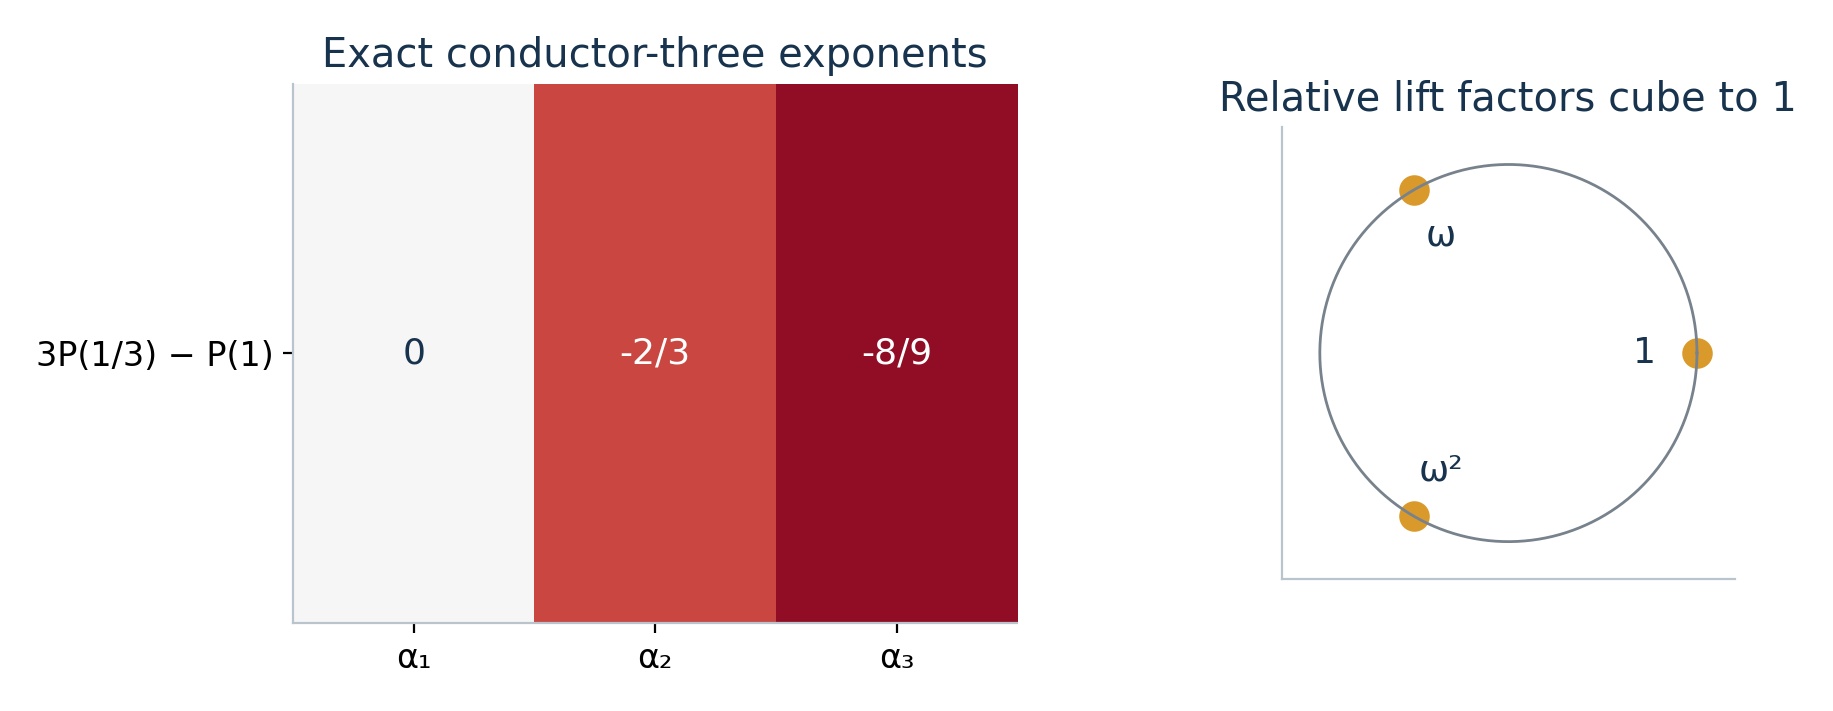
\includegraphics[width=.96\linewidth]{figures/16_cube.png}\caption{For $P(z)=\alpha_1z+\alpha_2z^2+\alpha_3z^3$, the exact coefficients of $3P(1/3)-P(1)$ are $0,-2/3,-8/9$. Cubing removes the possible relative logarithm-lift factor. This illustrates the analytic identity \eqref{eq:cube}, not an arithmetic evaluation.}\label{fig:cube}\end{figure}

\subsection{The repaired conjugation quotient and its boundary}
For $f^\#(z)=\overline{f(\overline z)}$, the canonical product $W_D^\#$ has the conjugate divisor. Hence
\begin{equation}\label{eq:regularized-conjugation}
 \frac{R/R^\#}{W_D/W_D^\#}
 =\frac{R_0}{\overline{R_0}}
 \exp\left(\sum_{j=1}^{3}(\alpha_j-\overline{\alpha_j})z^j\right).
\end{equation}
This is entire and nowhere zero, with modulus one on the real axis. It cancels all unmatched divisor orders by a canonical meromorphic factor. That factor is not a holomorphic-unit gauge or a finite theta section. Regularity on the scalar plane does not establish periodic descent to $\mathbb T^3$, identify a based multiplier with $U_\Gamma/U_{\rm alg}$, or supply the principal-norm coboundary of Section~\ref{sec:rigidity}. Those remain distinct obligations.
